\documentclass[11pt,letterpaper,boxed]{hmcpset}
\usepackage{fullpage}
\setlength{\parskip}{6pt}
\setlength{\parindent}{0pt}
\usepackage[margin=1in]{geometry}
\usepackage{graphicx}
\usepackage{enumerate}
\usepackage{marvosym}
\usepackage{amssymb}
\usepackage{wasysym}
\usepackage{gensymb}
\usepackage{mathrsfs}
\usepackage{scrextend}
\usepackage{mathtools}
\usepackage{pgfplots}
\usepackage{xspace}

\name{Name $\rule{4cm}{0.15mm}$}
\class{Physics 51 Section $\rule{.5cm}{0.15mm}$ Box \# $\rule{1cm}{0.15mm}$}
\assignment{Problem Set 6}
\duedate{15 October 2018}

\begin{document}

%\begin{center}
\noindent\textbf{Collaborators:} 
%\end{center} 

%\problemlist{}

\begin{problem}[HRK P32.6]
Figure 32-40 shows an arrangement used to measure the masses of ions. An ion of mass \textit{m} and charge $+q$ is produced essential at rest in source \textit{S} a chamber in which gas discharge is taking place. The ion is accelerated by potential difference $\Delta V$ and allowed to enter a magnetic field $\vec{B}$. In the field it moves in a semicircle, striking a photographic plate at distance x from the entry slit. Show that the ion mass \textit{m} is given by
$$ m =\frac{B^2q}{8 \Delta V}x^2$$
\begin{center}
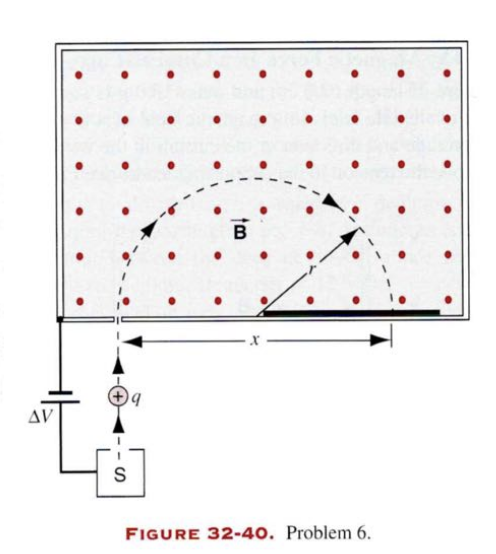
\includegraphics[scale=.6]{32-40.png}
\end{center} 
\end{problem}

\begin{solution}
\vfill
\end{solution}
\newpage

\begin{problem}[HRK 33.24 Solo]
Figure 33-50 shows a long wire carrying a current $i_1$ The rectangular loop carries a current $i_2$. Calculate the resultant force acting on the loop. Assume that $a= 1.10$ cm, $b= 9.20$, $L=32.3 cm$, $i_1=28.6$A, and $i_2=21.8$ A.
\begin{center}
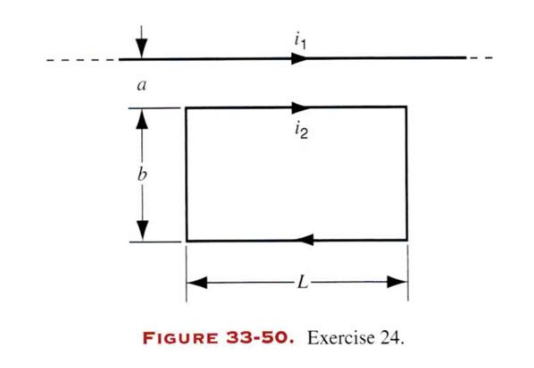
\includegraphics[scale=0.6]{33-50.png}
\end{center}
\end{problem}

\begin{solution}
\vfill
\end{solution}
\newpage

\begin{problem}[3. ]
Consider a rectangular wire loop of sides \textit{a} and $b$, carrying current $i$. The loop is oriented as shown, with its normal direction at an angle $\theta$ to a constant magnetic field $\vec{B}$. Calculate the torque exerted on the loop around its center, and show that the result can be written as $\vec{\tau} = \vec{\mu} \times \vec{B}$ where $\vec{\mu}$ is defined as the dipole moment of the loop equal to $iA\hat{\textbf{n}}$ where $A$ is the area of the loop. (It turns out that this relationship hold for loops of \textit{any} shape.) \textit{This result may be useful in Problem 4!}
\begin{center}
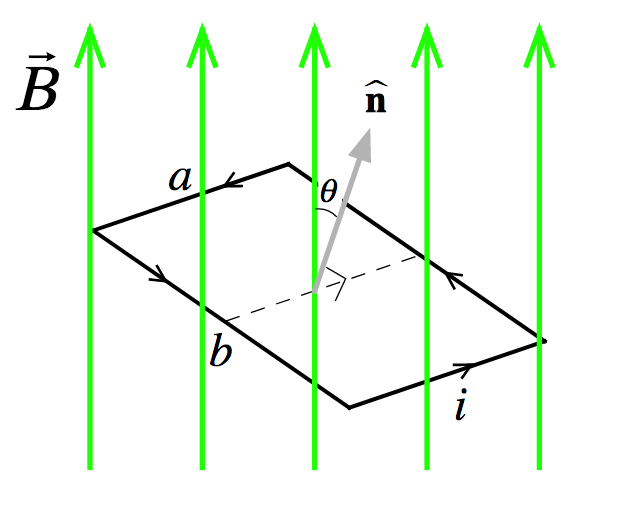
\includegraphics[scale=.6]{3.png}
\end{center}
\end{problem}

\begin{solution}
\vfill
\end{solution}
\newpage

\begin{problem}[HRK P32.19]
Figure 32-45 shows a wooden cylinder with a mass $m= 262$ g and a length $L= 12.7 cm$ with $N = 13$ turns of wire wrapped around it longitudinally, so that the plane of the wire loop contains the axis of the cylinder. What is the least current through the loop that will prevent the cylinder from rolling down a place inclined at an angle $\theta$ to the horizontal in the presence of a vertical uniform magnetic field of $477 mT$, if the plane of the windings is parallel to the inclined plane?
\begin{center}
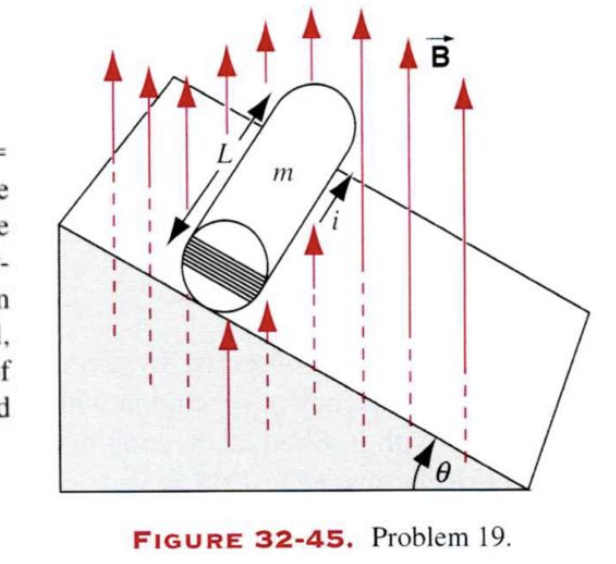
\includegraphics[scale=.6]{32-45.png}
\end{center}
\end{problem}

\begin{solution}
\vfill
\end{solution}
\newpage

\begin{problem}[HRK E33.13]
Consider the circuit of Fig. 33-42. The curved segments are arcs of circles of radii $a$ and $b$. The straight segements are along the radii. Find the magnetic field $\vec{\textbf{B}}$ at $P$, assuming a current $i$ in the circuit
\begin{center}
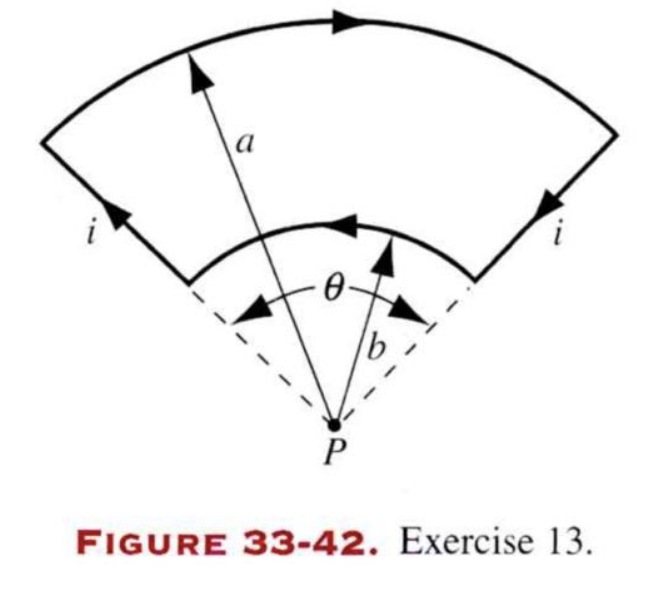
\includegraphics[scale=0.6]{33-42.png}
\end{center}
\end{problem}

\begin{solution}
\vfill
\end{solution}

\end{document}
